\documentclass{article}
\usepackage[utf8]{inputenc}
\usepackage[margin=1.2in]{geometry}
\usepackage{hyperref}

\PassOptionsToPackage{usenames,dvipsnames,svgnames}{xcolor}  
\usepackage{tikz}
\usetikzlibrary{arrows,positioning,automata}

\usepackage{natbib}
\usepackage{graphicx}
\usepackage{amsmath}
\usepackage{listings}
\usepackage{xcolor}


\definecolor{codegreen}{rgb}{0,0.6,0}
\definecolor{codegray}{rgb}{0.5,0.5,0.5}
\definecolor{codepurple}{rgb}{0.58,0,0.82}
\definecolor{backcolour}{rgb}{0.95,0.95,0.92}
\definecolor{deepblue}{rgb}{0,0,0.5}
\definecolor{deepred}{rgb}{0.6,0,0}
\definecolor{deepgreen}{rgb}{0,0.5,0}

\lstdefinestyle{mystyle}{
    backgroundcolor=\color{white},   
    commentstyle=\color{codegreen},
    keywordstyle=\color{deepblue},
    numberstyle=\tiny\color{codegray},
    stringstyle=\color{deepgreen},
    emph={Agent,__init__,act,self,union,exists, scope},
    emphstyle=\color{deepred},
    basicstyle=\ttfamily\footnotesize,
    breakatwhitespace=false,         
    breaklines=true,                 
    captionpos=b,                    
    keepspaces=true,                 
    numbers=left,                    
    numbersep=5pt,                  
    showspaces=false,                
    showstringspaces=false,
    showtabs=false,                  
    tabsize=3
}

\lstset{style=mystyle}

\title{\vspace{-2 cm} Universidade Federal de Ouro Preto \\ BCC 325 - Inteligência Artificial \\ Prova 2}
\date{}


\begin{document}

\maketitle

\vspace{-2 cm}
\begin{enumerate}

%Regressão Linear
\item Considere a solução de uma regressão linear obtida pelo método dos mínimos quadrados dada por $\mathbf{w} = (X^{t}X)^{-1}X^t\mathbf{y}$, e responda:
\begin{enumerate}
    \item O que represente o vetor $\mathbf{w}$?
    \item O que represente a matriz $\mathbf{X}$?
    \item O que representa o vetor $\mathbf{y}$?
    \item Como essa equação é derivada?
    \item É possivel utilizar este método para resolver problemas em que a relação entre variável dependente (o alvo), $y$, e as variáveis independentes (atributos de entrada), $\mathbf{x}$, não é linear? Como?  
\end{enumerate}

\item Considere os dados representados na figura abaixo:

    \begin{figure}[!ht]
        \centering
        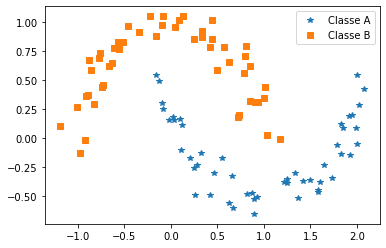
\includegraphics[width=0.41\textwidth]{moons.png}
    \end{figure}
    
    \begin{enumerate}
        \item É possível resolver este problema com um aplicação direta do algoritmo de regresão logística? Explique.
        \item O que poderia ser feito para que este problema possa ser resolvido com regressão logística?
    \end{enumerate}

\item Considere a base de dados abaixo:

\begin{table}[h!]
    \centering
    \begin{tabular}{|c|c|c|}
    \hline
    \textbf{Atributo1} & \textbf{Atributo2} & \textbf{Classe} \\
    \hline
    1 & 2 & Classe1 \\
    2 & 3 & Classe1 \\
    3 & 4 & Classe2 \\
    4 & 5 & Classe2 \\
    5 & 20 & Classe1 \\
    6 & 30 & Classe1 \\
    7 & 40 & Classe2 \\
    8 & 50 & Classe2 \\
    \hline
    \end{tabular}
    \caption{Exemplo de base de dados}
    \label{tab:exemplo}
\end{table}

\begin{enumerate}
    \item Calcule o gini para a condição $Atributo1 \leq 4.5$. $I_{G}(p) = 1 - \sum_{i=1}^{J} p_{i}^{2}$
    \item Quais seriam condições ótimas, em relação ao gini, após selecionarmos como raíz da árvore de decisão o critério $Atributo1 \leq 4.5$. Desenhe essa árvore.
    \item Indique uma forma de controlar o overffiting de uma árvore de decisão e explique por quê o overfitting é reduzido com esta técnica. 
\end{enumerate}



\item Como escolhemos a função de custo (perda) de uma rede neural artificial? Justifique.

\item Quais as vantagens do algoritmo de busca em largura sobre o algoritmo de busca em profundidade? E quais as desvantagens?

\item Quando devemos utilizar o algoritmo de busca A*?

\end{enumerate}

\end{document}

